%%%%%%%%%%%%%%%%%%%%%%%%%%%%%%%%%%%%%%%%%%%%%%%%%%%%%%%%%%%%%%%%%%%%%%%%%%%%%%%%
%2345678901234567890123456789012345678901234567890123456789012345678901234567890
%        1         2         3         4         5         6         7         8

\documentclass[letterpaper, 10 pt, conference]{ieeeconf}  % Comment this line out if you need a4paper

%\documentclass[a4paper, 10pt, conference]{ieeeconf}      % Use this line for a4 paper

\IEEEoverridecommandlockouts                              % This command is only needed if
% you want to use the \thanks command

\overrideIEEEmargins                                      % Needed to meet printer requirements.

%In case you encounter the following error:
%Error 1010 The PDF file may be corrupt (unable to open PDF file) OR
%Error 1000 An error occurred while parsing a contents stream. Unable to analyze the PDF file.
%This is a known problem with pdfLaTeX conversion filter. The file cannot be opened with acrobat reader
%Please use one of the alternatives below to circumvent this error by uncommenting one or the other
%\pdfobjcompresslevel=0
%\pdfminorversion=4

% See the \addtolength command later in the file to balance the column lengths
% on the last page of the document

% The following packages can be found on http:\\www.ctan.org
\usepackage{graphics} % for pdf, bitmapped graphics files
\usepackage{epsfig} % for postscript graphics files
%\usepackage{mathptmx} % assumes new font selection scheme installed
%\usepackage{times} % assumes new font selection scheme installed
\usepackage{amsmath} % assumes amsmath package installed
\usepackage{amssymb}  % assumes amsmath package installed
\usepackage{multicol}
\usepackage[bookmarks=true]{hyperref}
\usepackage{xcolor}
\usepackage{booktabs}
\usepackage{graphicx}
\usepackage{svg}
%\usepackage{subfigure}
\usepackage{subcaption}

\usepackage[backend=bibtex,style=ieee,natbib=true,mincitenames=1,maxcitenames=2]{biblatex}
\addbibresource{refs.bib}

\newcommand{\etal}{\textit{et al}. }
\newcommand{\ie}{\textit{i}.\textit{e}., }
\newcommand{\eg}{\textit{e}.\textit{g}. }

\newcommand{\Varun}[1]{\textcolor{green}{Varun: #1}}
\newcommand{\Shivika}[1]{\textcolor{red}{Shivika: #1}}
\newcommand{\Yuri}[1]{\textcolor{yellow}{Yuri: #1}}

% Increaset spacing in table rows
\renewcommand{\arraystretch}{1.1}


\title{\LARGE \bf
    Simultaneous Trajectory Estimation and Learning
}


\author{Shivika Singh$^{1}$, Yuri Ahn$^{1}$, Varun Agrawal$^{1}$% <-this % stops a space
    % \thanks{*This work was not supported by any organization}% <-this % stops a space
    \thanks{$^{1}$College of Computing, Georgia Institute of Technology, Atlanta, GA 30332 USA. Author names in lastname reverse alphabetical order.
        {\tt\small \{ssingh794,yahn41,varunagrawal\}@gatech.edu}
        GTIDs: 903841199, 903227172, 902994361}%
}


\begin{document}
    
    
    
    \maketitle
    \thispagestyle{empty}
    \pagestyle{empty}
    
    
    %%%%%%%%%%%%%%%%%%%%%%%%%%%%%%%%%%%%%%%%%%%%%%%%%%%%%%%%%%%%%%%%%%%%%%%%%%%%%%%%
    \begin{abstract}
    To deploy robots in general, dynamic environments, it is imperative for them to be able to learn new skills and execute these task trajectories in a safe, stable and reliable fashion. Recent work has combined Learning from Demonstration with classical control techniques to achieve state of the art results while maintaining theoretical guarantees. However, these works assume the availability of expert demonstrations and are poorly equipped to handle suboptimality. In this work, we propose to tackle this solution by leveraging Gaussian Processes as a probabilistic representation of demonstrations and coupling it with the RMPflow framework for motion generation. The flexibility of Gaussian Processes allows us to incorporate ideas from inverse reinforcement learning, and we can sample pseudo-expert trajectories from the estimated posterior. We demonstrate empirical results on the LASA handwriting dataset, showing a proof-of-concept of our work. 
    \end{abstract}
    
    \section{Introduction}

The goal of roboticists is to enable general-purpose robots that can work with human collaborators to achieve greater efficiency and productivity than the current status quo.

To accomplish the task set for the robot, two criteria must be satisfied: the robot should be able to succeed at the task in new environments outside of the scope for which it was originally programmed, and it should be able to perform the task safely, reliably while allowing for failure analysis.

Learning-based techniques have emerged as a major paradigm to enable robot adaptivity. Learning from demonstrations (LfD)~\cite{Argall09ras} in particular is a powerful approach to teach robots new skills or the ability operate in new environments. This enables the robot to achieve task success with a small number of demonstrations as per a demonstrator-determined metric.
Safety, reliability, and interpretability are important characteristics required to allow for the widespread deployment of robotics. Safety and reliability can help invoke confidence in the general masses in the sustainability of robot solutions, while interpretability can aid in debugging the failure cases that may occur, and allow for putting in appropriate safeguards. These characteristics have been extensively researched in the robotic control literature, and many theoretical and practical guarantees can be made.

To get the best of both worlds, we leverage the recently proposed RMPFlow framework~\cite{Cheng21tase} for generating stable, locally reactive trajectories in non-Euclidean spaces (or manifolds). RMPFlow operates on subtask manifold spaces where each subtask can be connected in a tree-based data structure. Using the calculus of Riemannian Motion Policies (RMPs), the optimal acceleration policies for each subtask can be combined to provide a globally optimal and stable policy, satisfying the second criteria detailed above. Alternatively, we can learn the subtask map and Riemannian metric for the RMP corresponding to the desired task~\cite{Rana20corl,Rana20ldc}, which RMPFlow can then combine optimally, thus achieving the first criteria. The structure imposed by the RMP also makes learning from a limited number of demonstrations viable, thus making it a natural fit for LfD techniques.

The current drawback of existing works leveraging learning with RMPflow is that they rely on expert demonstrations. The teacher in each of these cases is assumed to be aware of the underlying robot structure and capabilities. This severely limits the widespread adoption of robotics due to the complexity and expense involved in training the task force. To address this shortcoming, we would like to accommodate non-expert, suboptimal trajectories in an intuitive way.

Gaussian Processes~\cite{Rasmussen04book} are a powerful mechanism for probabilistically representing trajectories~\cite{vanWaveren22manuscript}. A Gaussian Process (GP) is a non-parametric model which represents a distribution over functions, where any subset of these function values is jointly gaussian. Due to their non-parametric nature, GPs are fully specified by the Gaussian Process prior and the data provided. GPs are also highly interpretable since their covariance functions (a.k.a. kernel) provide structure and encode knowledge about the data distribution.

In this work, we propose to leverage Gaussian Processes with an appropriate kernel definition to accommodate suboptimal demonstration trajectories. By computing the posterior of the GP, we can learn the optimal mean trajectory for the task while being flexible to newly provided trajectories.
To train the RMP for use in RMPflow, we can sample trajectories from the posterior GP and use that as our set of expert demonstrations. The posterior GP can also provide us with highly variable trajectories, which have been shown to improve policy learning~\cite{Duan17neurips}.

We show results on a simple benchmark dataset~\cite{Khansari-Zadeh11tro}, where we train a Gaussian Process to estimate the posterior trajectory from a set of sample demonstrations. This GP is then sampled to provide ``pseudo''-expert trajectories which are used to train the RMP node in RMPflow to give us the final learned policy. We empirically demonstrate the ability to recreate the trajectories in the benchmark dataset as a proof of concept of our method.


% %===============================================================================
% \vspace{-1em}
% \section{Description}

% To generate a stable, reactive robot policy, we leverage RMPFlow~\cite{Rana20corl}. RMPFlow provides a mathematically sound framework for generating guaranteed Lyapunov stable and reactive policies by leveraging Riemannian Geometry. This is related to prior work in motion policy generation such as DMP~\cite{Schaal06amam} but generalize over methods such as DMP and Model Predictive Control~\cite{Ratliff18arxiv}, making them a state-of-the-art framework for policy generation.

% We propose to leverage the framework described by~\cite{Rana20corl}, to learn a controller from potentially suboptimal demonstrations. This is accomplised by learning the Riemannian Motion Policy (RMP) potential functions $\Phi$ and the corresponding Riemannian metric \textbf{M}.
% %This is similar to learning the potential functions over classical impedance control~\cite{KhansariZadeh17ar} but with the added benefits of the Riemannian Geometry, providing us with reactive, safe, stable and hopefully optimal controllers.

% A key drawback of~\cite{Rana20corl} is that all the trajectories provided to the algorithm are given by a human expert. Thus the demonstration suboptimality is controlled to a certain extent as the selected nominal trajectory is from the dataset of expert trajectories and will be close to the other trajectories in the task space, something which may not be true in many real-world applications.

% Instead of picking one trajectory from the dataset as the nominal trajectory (via the use of Dynamic Time Warping), we propose to model the nominal trajectories throuhgh the use of a Gaussian Process. A gaussian process (GP) is a mathematical framework for probabilistically modeling continuous time functions. Here each function is the trajectory $\zeta(t)$ indexed by time $t$. GPs have seen significant application in the robotics community as a way to represent continuous-time trajectories~\cite{Barfoot14rss,Dong18icra} and thus form a natural choice for our proposed method. Additionally, GPs possess desirable properties such as exact sparsity and a low data requirement. Since GPs are estimated via a posterior probability, we can further expand their utilities and constraints by adding information via the priors (e.g. Mutual Information).

% As a stretch goal, a question we would like to answer as well is whether this framework can also handle heterogenous demonstrations. Given $N$ different datasets, each for a specific skill, it would be interesting to understand the pros and cons of our approach in such a heterogenous regime.

% %===============================================================================
% \section{Data}

% \subsection{Simulation}

% To establish correctness of our algorithm, we wish to first execute our proposed framework on a simple object push task in simulation. The goal of this task is to teach a manipulator to push a block over a line from few, teleoperated demonstrations. We can add further constraints such as performing the same task with clutter.

% For a real world task, we propose to use Assistive Gym's Robot Feeding Task as a dataset.
% Assistive Gym~\cite{Erickson20icra} provides a simulated environment for Robot Healthcare integrated into OpenAI's Gym environment.
% Feeding is a non-trivial task due to various considerations such as the human in the loop as well as voluntary and involuntary motion from the human to whom assistance is being provided. We believe this task can demonstrate the benefits of our approach very well.

% \subsection{Human Data}

% As a stretch goal, if time permits, we would like to collect data from human demonstrations as well for a simple pick and place task. However, we wish to first see success in the simulation cases.

% %===============================================================================

% \section{Data Collection Protocol}

% \subsection{Simulation}

% For both sets of simulated tasks, data will be collected via teleoperation. To encourage suboptimality, each of our team members will provide demonstrations without seeing each other's provided demonstrations. If need be, we will recruite friends for additional variance in the dataset.

% \subsection{Human Data}

% Human demonstrations would be collected either via Teleoperation or Kinesthetic Teaching of a Franka Arm or a Sawyer robot since they are robots available to us at Georgia Tech.

% %===============================================================================

% \section{Expected Outcome}

% The expected outcome of our approach is that we are able to learn a policy generated from RMPFlow which achieves the proposed tasks successfully and is adaptable to both dynamic environment changes as well as new information provided (via the Gaussian Process prior or the RMP constraints)., given suboptimal demonstrations.

% Our hope is that the use of RMPFlow implies lower risk to humans during deployment, but a potential risk is the gap between our provided demonstrations and the expectation of the end-users.

% %===============================================================================

% \section{Identification of Benchmark}

% We will compare our framework to the one proposed in~\cite{Rana20corl}. A simple metric we can use is ratio of task success as well as time for task execution.

% %===============================================================================

% \section{Timeline}
% \begin{itemize}
%     \item Week 1 Setup all the necessary software.
%     \item Week 2 Data collection for push task and Assistive Gym task.
%     \item Week 3 Project design and implementation.
%     \item Week 4-6 Evaluation and debugging.
%     \item Week 7 Report and presentation creation.
% \end{itemize}

    \section{Related Works}

    % Background on GP, RMPFlow
\section{Preliminaries}

\subsection{Gaussian Processes}
A Gaussian Process (GP) is defined as a collection of random variables, any finite number of which have a joint Gaussian distribution~\cite{Rasmussen04book}.
A GP is fully defined by its mean function $m(t)$ and covariance function (or kernel) $k(t,t')$ over the distribution of functionals $f(x)$ as: 
\begin{center}$m(t)= \mathbb{E}[f(t)]$  \\
\medskip
$k(t,t') = \mathbb{E}[(f(t)  - m(t)) ((f(t')-m(t')))]$
\end{center} 
By definition, $k(t,t')$ is a symmetric and positive semi-definite function. $f(x)$ represents the random variables at input $x$, where $x$ is often time in the case of robot trajectories, which we adopt as well~\cite{Nguyen21arxiv}.
% For Multivariate Gaussian distributions, the mean is the vector-valued expectation of the data. Similarly, the covariance matrix is a symmetric and positive semi-definite matrix~\cite{Nguyen21arxiv} representing the correlation between the data samples.
The kernel in a Gaussian Process can be a single covariance function or a combination of kernels. A commonly used kernel is the Squared Exponential (SE)/Radial Basis Function (RBF) Kernel, which is both stationary and smooth. This kernel is defined by:
\begin{center}
    $k_{SE}(x,x') = \sigma^2 exp(-\frac{(x-x')^2}{2l^2})$
\end{center}
where $l$ is the length scale and $\sigma^2$ is the variance~\cite{Duvenaud14thesis}. A kernel function $k(x,x')$ generally consists of some hyperparameters that can be estimated by maximizing the log marginal likelihood:
\[ \log{p(y|X)} = \frac{1}{2} y^{T} (K+\sigma_{n}^{2}I)^{-1}y - \frac{1}{2} \log |K+\sigma_{n}^{2}I| - \frac{n}{2} \log 2\pi\]

Unlike Simple Gaussian Processes, Multitask Gaussian Processes take a set of input values and predict multiple tasks that share the same input and simultaneously learn a shared covariance function~\cite{Bonilla07neurips}. This enables learning of inter-task similarities in the covariance matrix. Multitask GPs can utilize exact inference methods or variational methods. Multitask GP causes the covariance matrix to potentially grow extremely large and exact inference requires the inverse of this matrix, which can become very computationally expensive. Variational or approximation methods help reduce the size of this covariance matrix by utilizing inducing points to represent the dataset with a much smaller set of data points, thus reducing the computational complexity.

\subsection{RMPflow}

A Riemannian Motion Policy is an acceleration policy that operates on smooth, differentiable (\ie Riemannian) manifolds.
It has associated with it a Riemannian Metric which determines the curvature of the geodesics on the manifold~\cite{Ratliff18arxiv}, allowing for the definition of locally reactive policies in non-Euclidean task spaces while accounting for abnormal trajectories, \eg holes in the space due to the presence of obstacles to avoid. RMPs are built upon the notion of Geometric Dynamical Systems and subsume prior work on dynamical systems for robot control such as DMPs~\cite{Ijspeert13nc} and ProMPs~\cite{Paraschos13neurips}. Moreover, they are Lyapunov stable and their enforced structure makes learning relatively easier.

RMPFlow~\cite{Cheng21tase} is a computational framework for automatically combining various RMP motion policies on various subtasks. RMPflow arranges the subtasks into a tree datastructure called the RMPtree where nodes represent the acceleration policy and Riemannian metric for the subtask space and the edges represent task maps from one task space to another. The tree structure allows for ease of task specification since each node represents a specific task objective, simplifying controller design. By utilizing the calculus of RMPs, RMPflow is able to optimally combining the motion policies in the child nodes to generate a globally optimal and stable policy which automatically handles the various subtask constraints.
    \section{Method}
    \section{Results}

\subsection{LASA Handwriting Dataset}
We used the LASA handwriting dataset which consists of a library of 2D handwriting motion trajectories~\cite{Khansari-Zadeh11tro}. There are 7 trajectories recorded for each handwriting motion. All the trajectories of a given hand motion start from different positions but end at the same position. Each trajectory consists of a set of states consisting of timestamp, $x$-position, $y$-position, $x$-velocity, $y$-velocity, $x$-acceleration, and $y$-acceleration. We are primarily interested in learning the position values for each timestamp along the trajectory because we can derive the velocity from the positions. Our framework was tested with the 'heee' handwriting motion.

\begin{figure*}[h!]
	\captionsetup{font=footnotesize}
	\centering

	\begin{subfigure}{0.45\textwidth}
		\label{fig:atlasrobot}
	    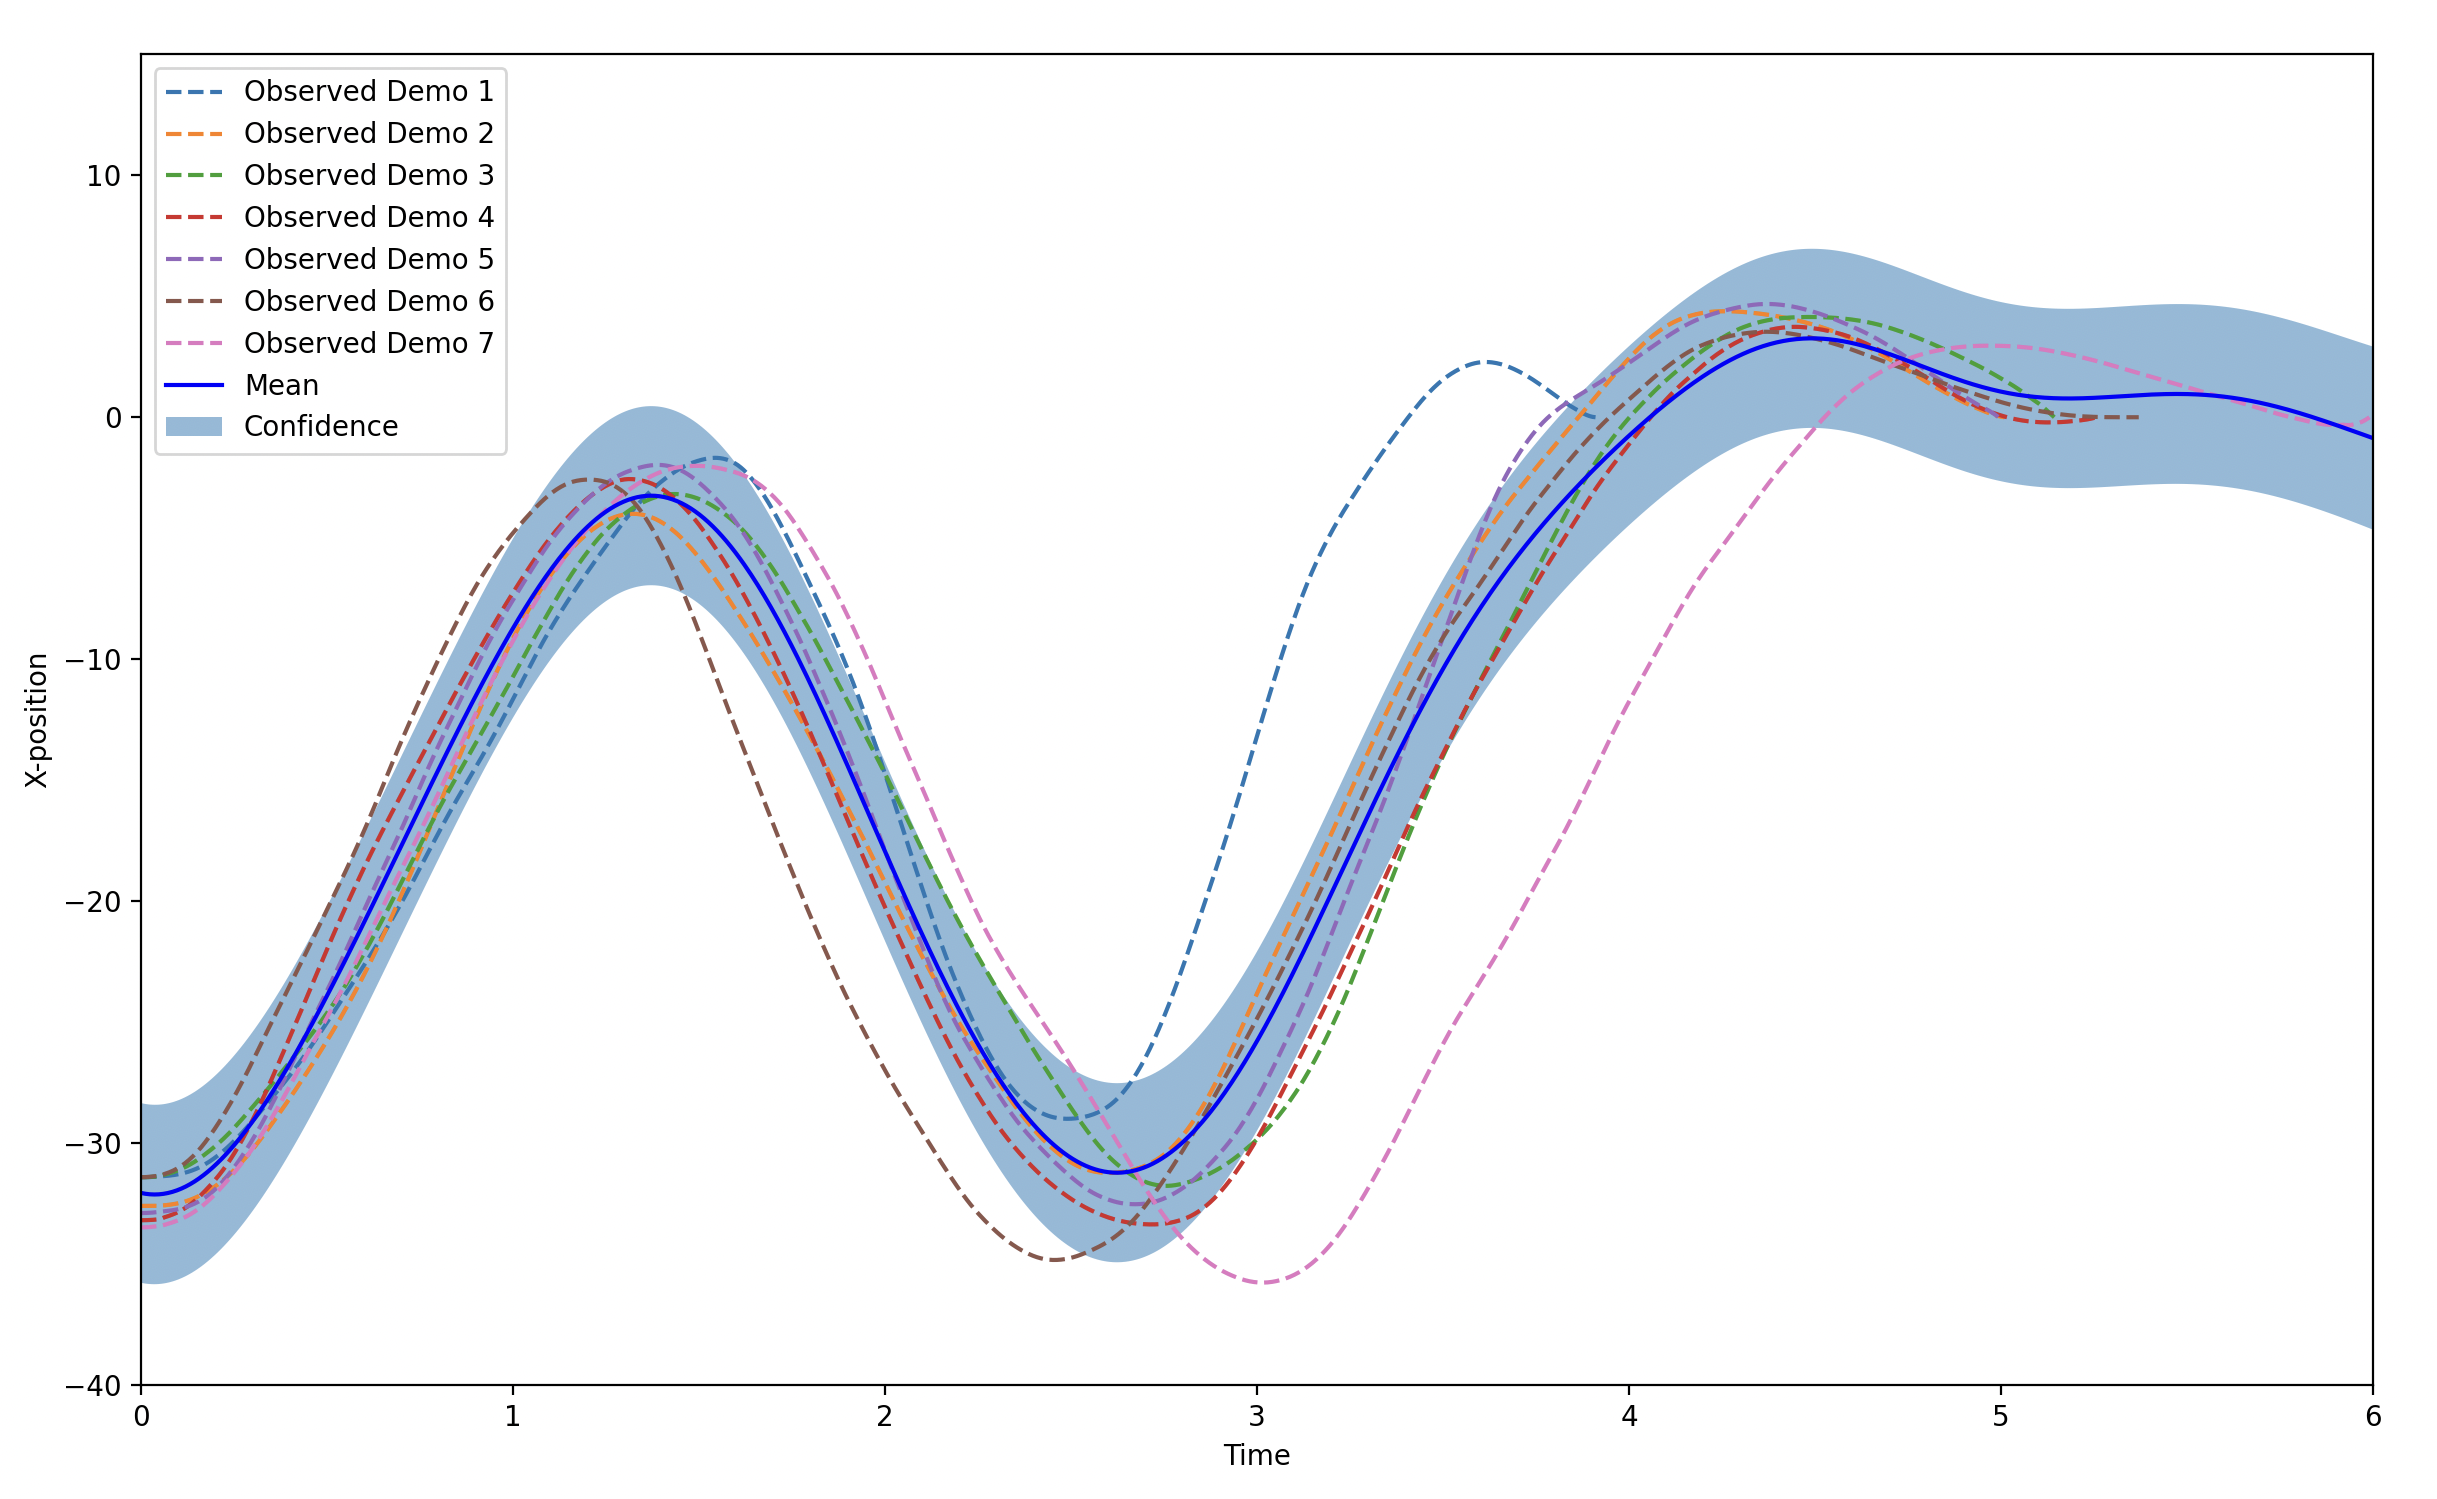
\includegraphics[width=\textwidth]{paper/images/X_time_Exact_GP_RBF.png}
		\caption{$x$ position as the task (output) and time $t$ as the input to the GP.}
	\end{subfigure}
	\begin{subfigure}{0.45\textwidth}
		\label{fig:atlas_traj_example}
		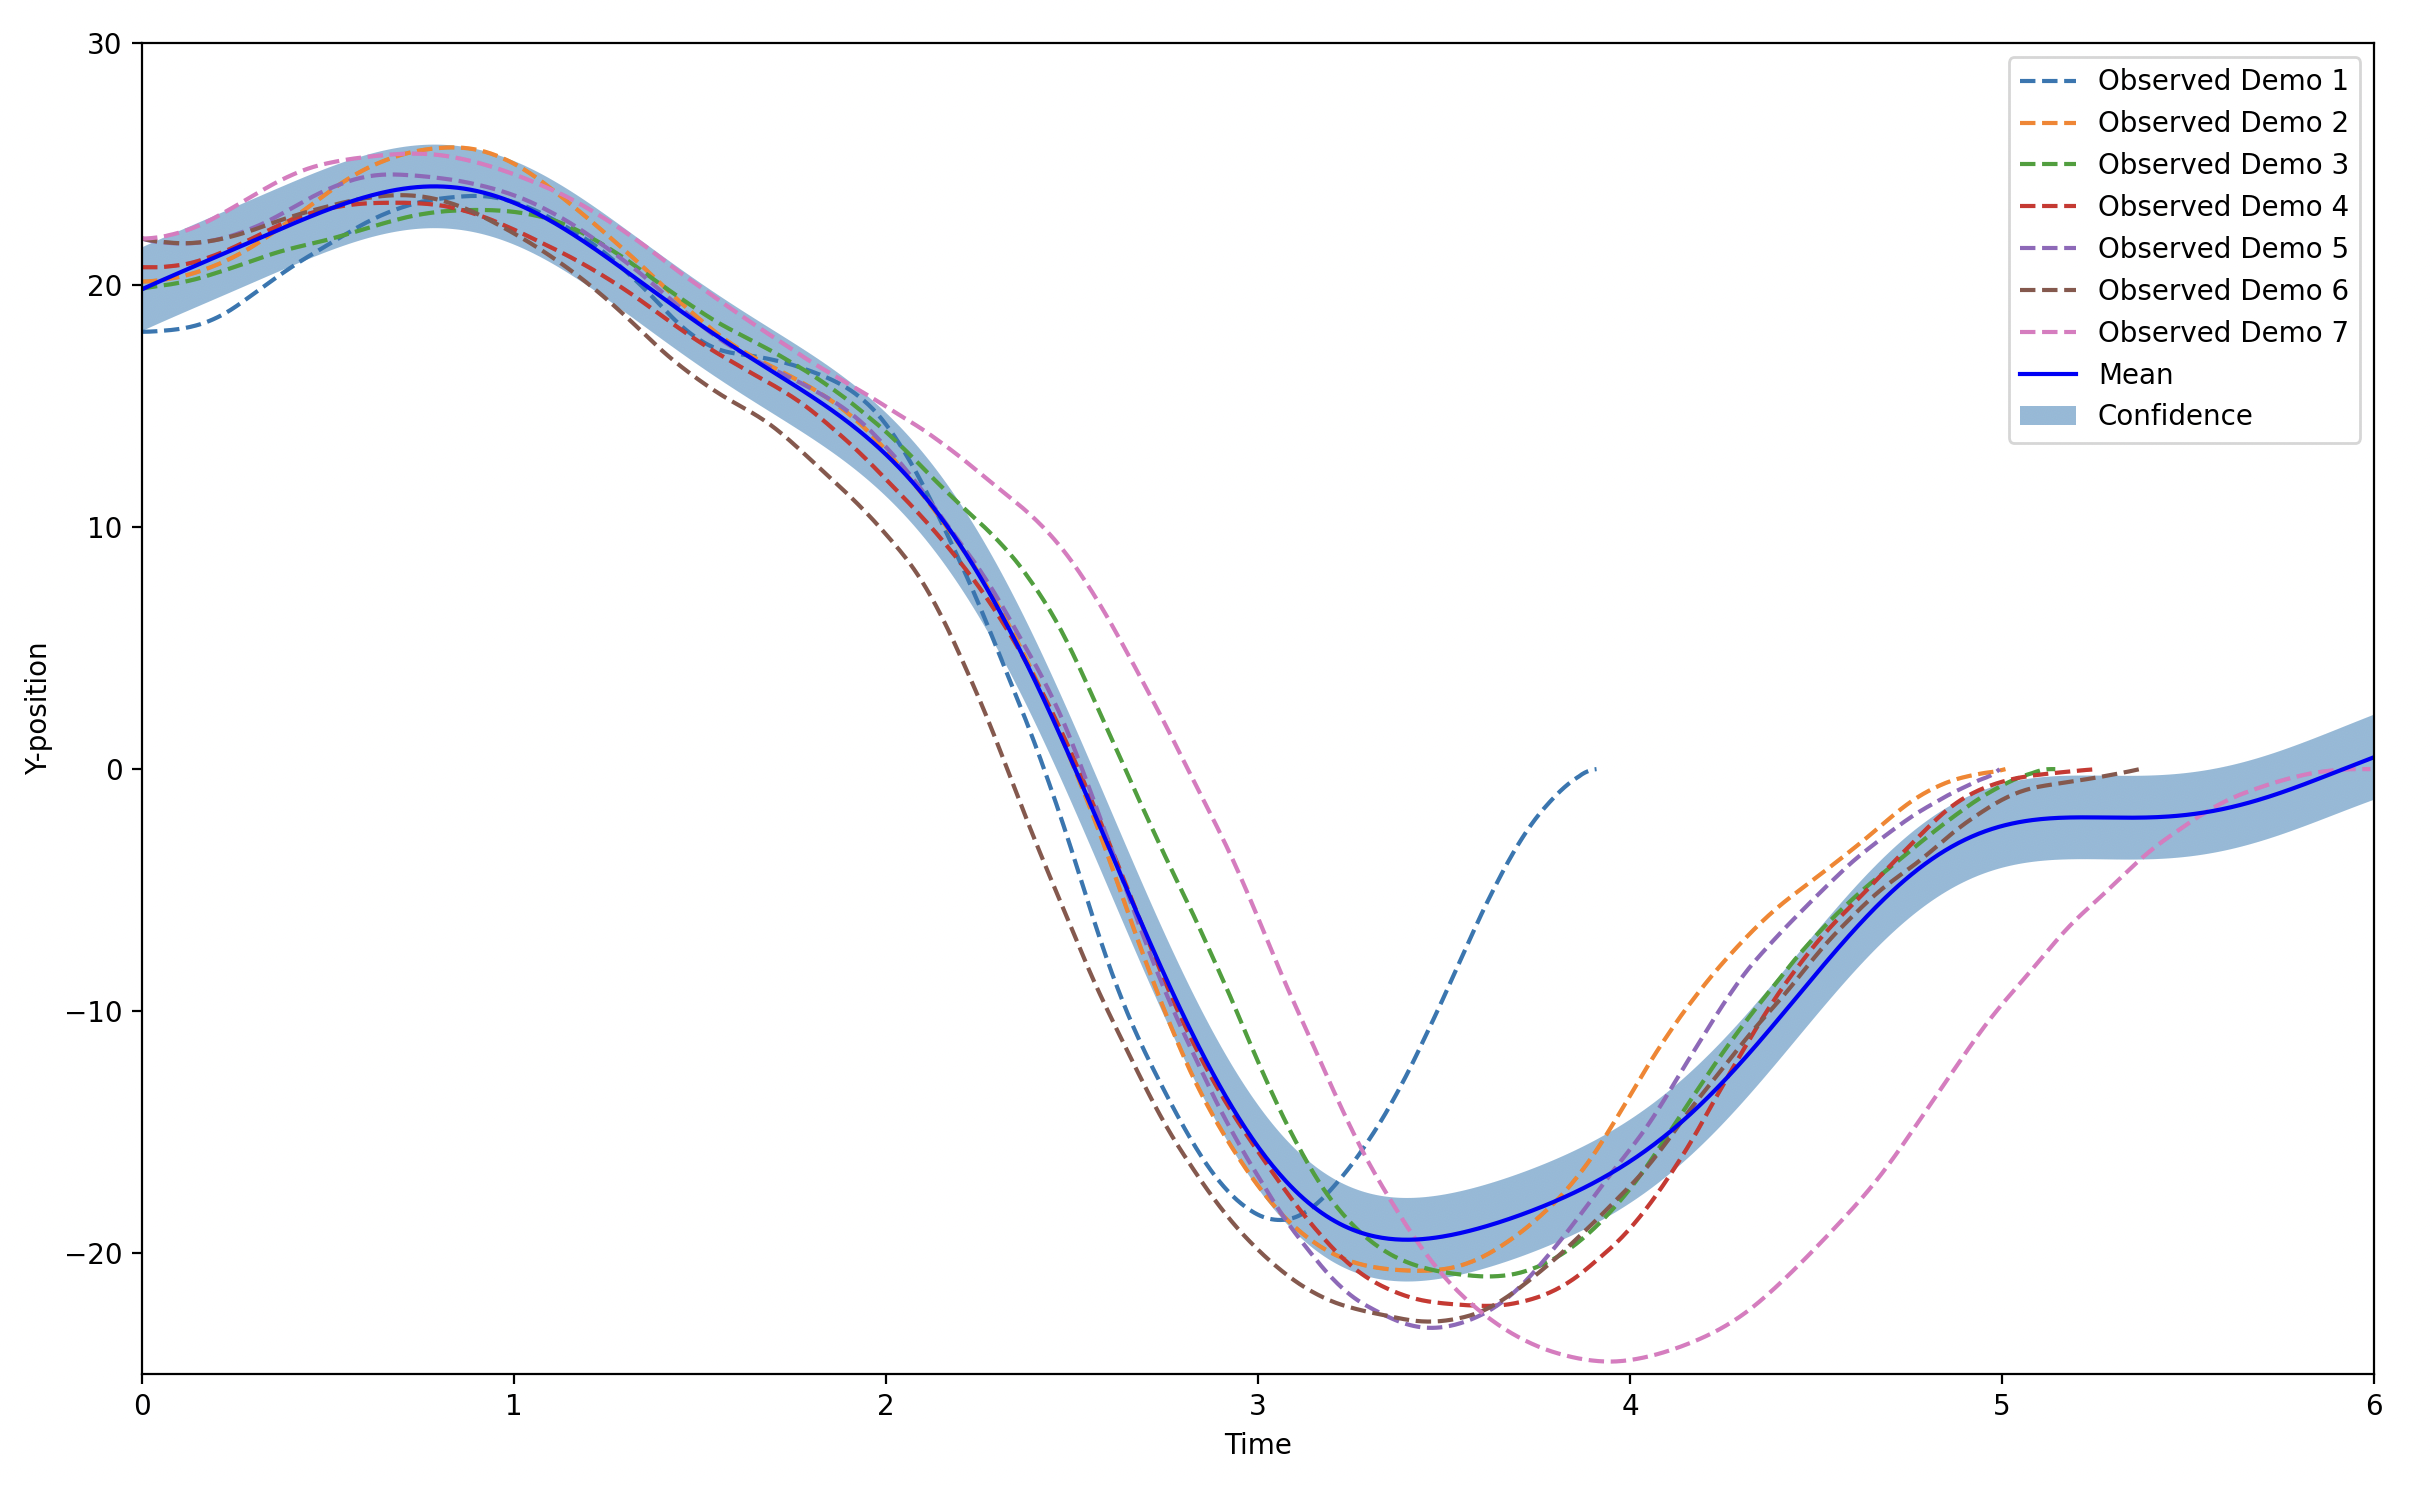
\includegraphics[width=\textwidth]{paper/images/Y_Time_Exact_GP.png}
		\caption{$y$ position as the task (output) and time $t$ as the input to the GP.}
	\end{subfigure}
	
	\caption{The 7 trajectories of the "heee" motion shape are shown in various colors. The posterior mean and confidence region are shown as the blue line and the blue shaded region respectively.}

    \label{fig:scalar_exact}

    \vspace{-2em}
\end{figure*}

\subsection{Trajectory Estimation}
We use the Radial Basis Function (RBF) kernel function in all of the following Gaussian Processes.

\begin{figure*}[t!]
    \captionsetup{font=footnotesize}
    \centering
    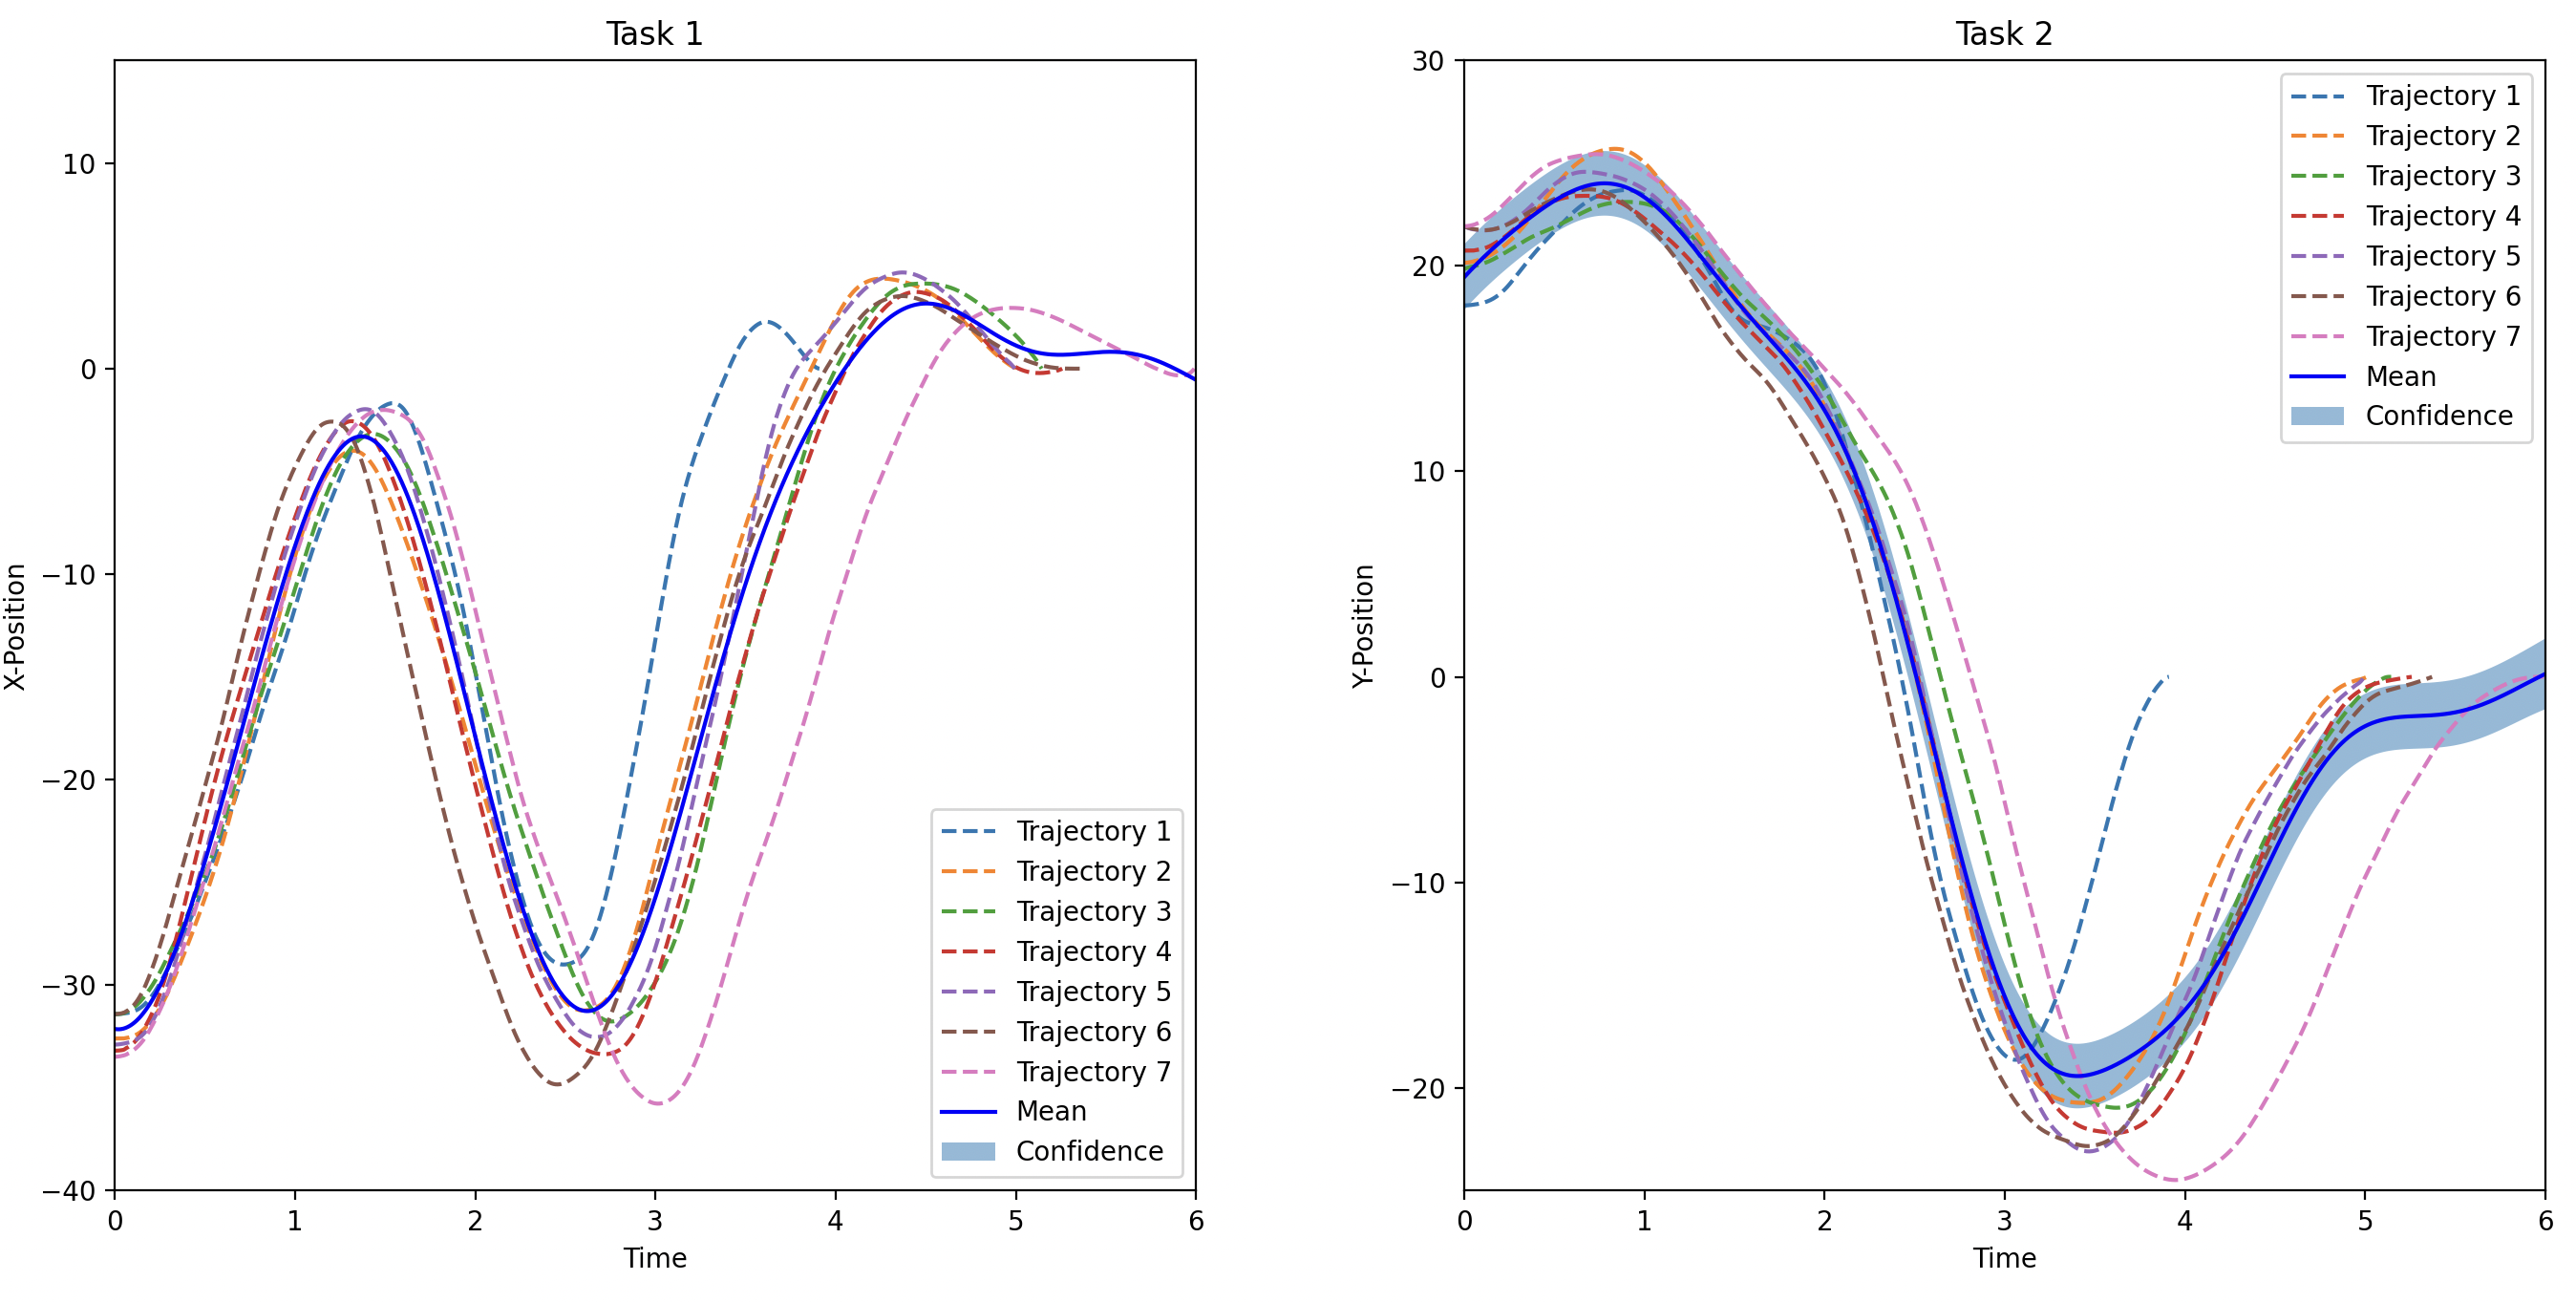
\includegraphics[width=\textwidth]{paper/images/Multi_Exact_GP.png}
    \caption{An example of 10 trajectories sampled from the posterior of the variational multi-output Gaussian process.}
    \label{fig:multitask_exact}
    \vspace{-2em}
\end{figure*}

\subsubsection{Gaussian Process with Exact Inference}
The Gaussian Process with exact inference can only map single-dimensional input to a single-dimensional output. Therefore, two Gaussian Processes were trained independently for predicting $x$-position from time input and $y$-position from time input. Figure~\ref{fig:scalar_exact} 1a shows the 7 trajectories of the "heee" motion shape for $x$ position as the task and time as input, the mean and the confidence region (two standard deviation above and below the mean). While training independent GPs gave good estimation for the mean and the confidence region, the inter-task covariance information was not encoded which motivated us to experiment with other GPs.

\begin{figure*}[t!]
    \captionsetup{font=footnotesize}
    \centering
    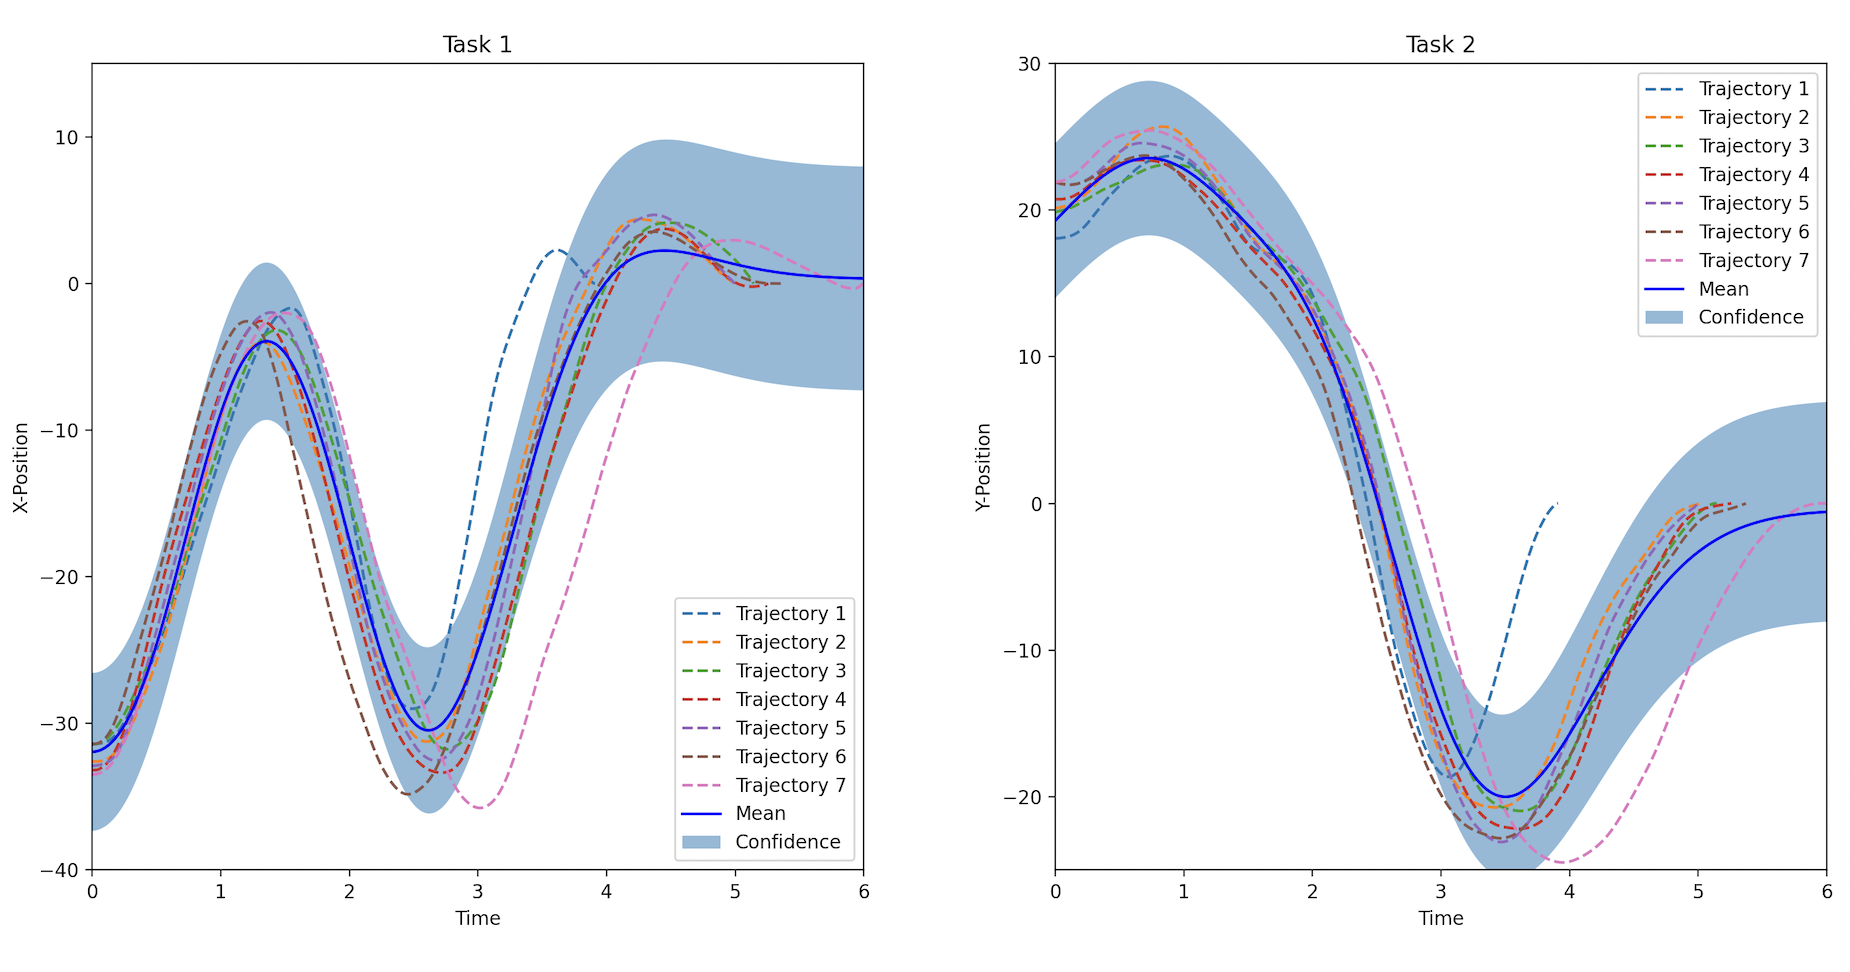
\includegraphics[width=\textwidth]{paper/images/VGP_RBFKernel.png}
    \caption{An example of a multi-output Gaussian process trained to estimate the trajectory distribution via Variational Inference.}
    \label{fig:multitask_approx}
    \vspace{-2em}
\end{figure*}


\begin{figure*}[h!]
    \captionsetup{font=footnotesize}
    \centering
    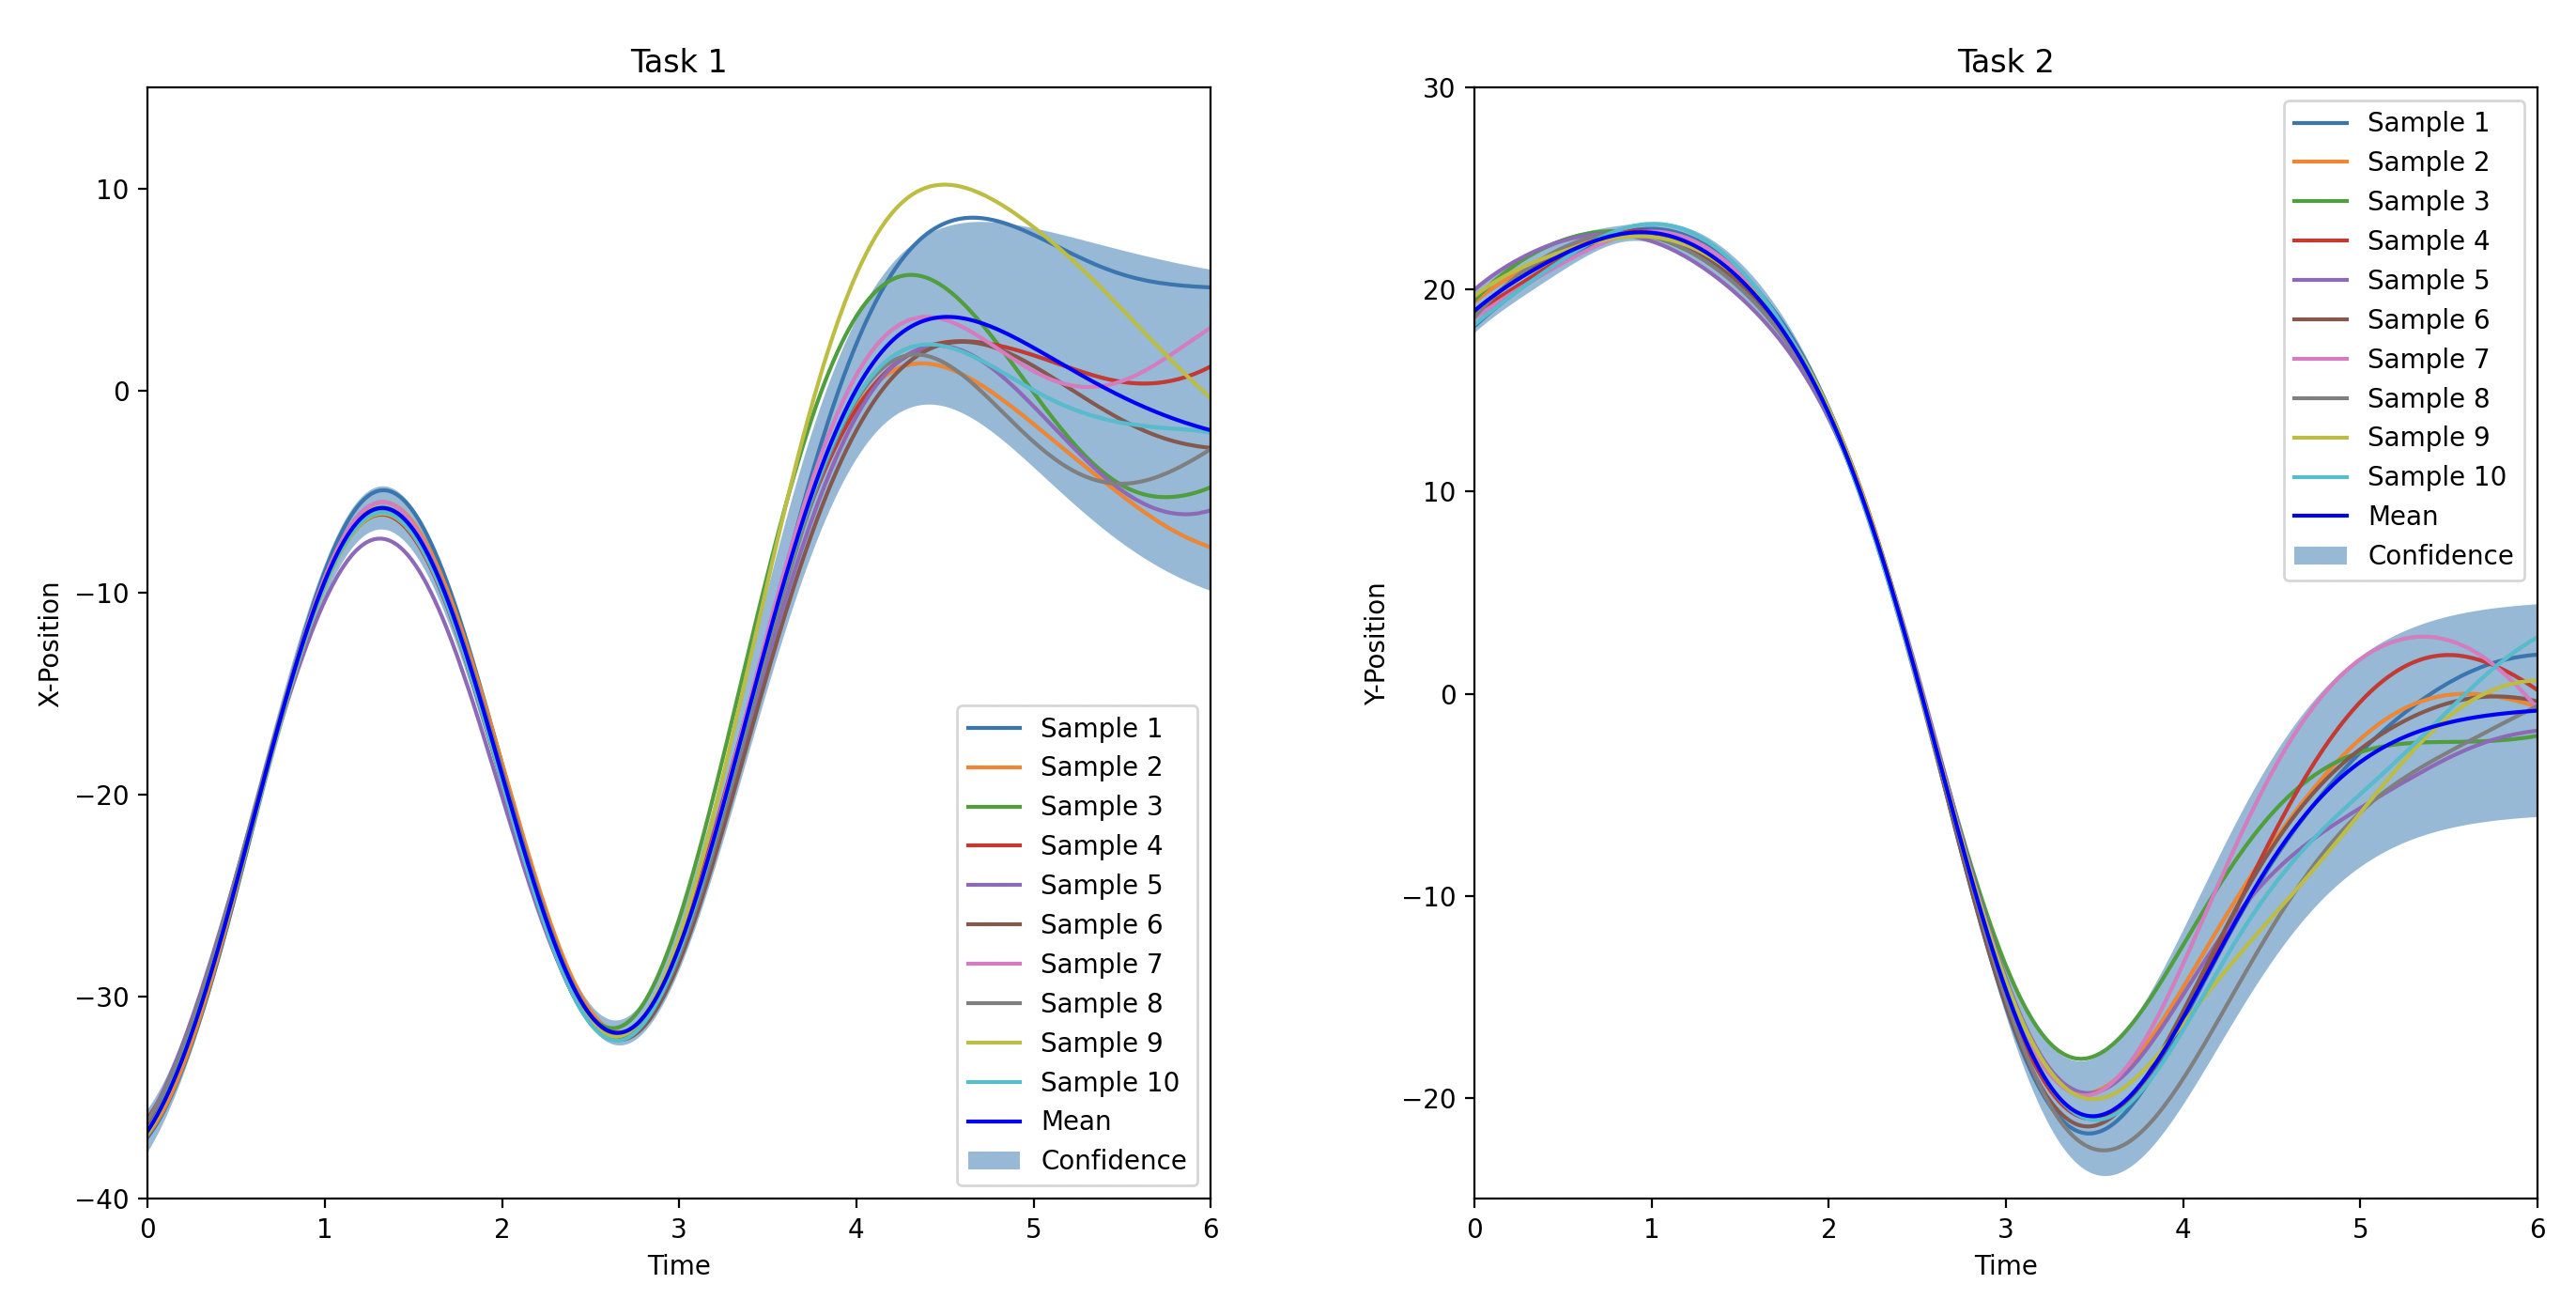
\includegraphics[width=\textwidth]{paper/images/VGP_RBF_sampling.png}
    \caption{An example of 10 trajectories sampled from the posterior of the variational multi-output Gaussian process.}
    \label{fig:multitask_sampling}
    \vspace{-2em}
\end{figure*}

\subsubsection{Multi-Output Gaussian Process with Exact Inference}
The Multi-Output Gaussian Processes can encode the inter-task covariance. We can directly use the time to predict the corresponding X and Y positions. However, due to the large dimensions of the $MN \times MN$ covariance matrix ($14000\times 14000$ in our case), the inverse of the covariance matrix was not being calculated correctly which lead to incorrect confidence values as visible in the left-most plot in Figure~\ref{fig:multitask_exact}. The covariance value was 0 for all pairs of input which lead to no confidence region.


\subsubsection{Variational Multi-Output Gaussian Process}
The Variational Multi-output Gaussian Process uses inducing points to reduce the size of the covariance matrix. We were successfully able to estimate the posterior mean and covariance as shown in Figure~\ref{fig:multitask_approx}. The estimated posterior was sampled to generate near-optimal trajectories (Figure~\ref{fig:multitask_sampling}) which will be used by the RMPFlow to learn the motion policy.

\subsection{Learning RMPs from GP Samples}

\begin{figure}[h!]
    \captionsetup{font=footnotesize}
    \centering
    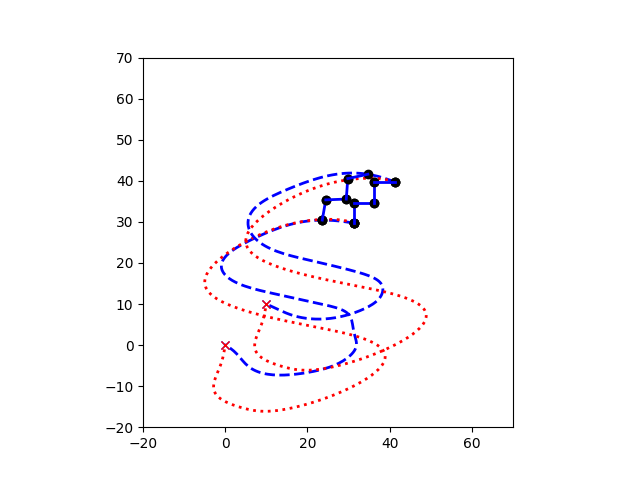
\includegraphics[width=\columnwidth]{paper/images/gp_sample_rmpflow.png}
    \caption{An example of an RMP learned for the ``Sshape'' trajectory in the LASA dataset.}
    \label{fig:gp_rmpflow}
    \vspace{-2em}
\end{figure}

In figure~\ref{fig:gp_rmpflow}, we showcase an example of a learned RMP motion policy which has been trained from samples of the Gaussian Process.
While not quite clean, the general ``S'' structure of the trajectory is reproduced and thus can be counted as a success.
We do believe, however, that there is a bug somewhere in the RMPflow code from the authors of~\cite{Rana20ldc} which we hope to remedy in the near future to generate the expected results.

    \section{Discussion}
    \section{Conclusion}
    
    
    
    \newpage
    \printbibliography
    
    
\end{document}
